\subsection{Introduction}

This section focuses on a class of approximate inference algorithms based on variational inference. The basic idea is to choose an approximation $q(x)$ from a tractable family of distributions and then make this approximation as close as possible to the true posterior $p^{\ast}(x)$. This reduces inference to an optimization problem.\\

We can use KL divergence to measure the distance between distributions. In particular, we use reverse KL to make the computation tractable.
\begin{equation}
    KL(q||p^{\ast}) = \sum_x q(x) \log \frac{q(x)}{p^{\ast}(x)}
\end{equation}
Let $\tilde{p}(x)=p^{\ast}(x)Z$ be the un-normalized distribution, then our objective function:
\begin{eqnarray}
    J(q) = KL(q||\tilde{p})= \sum_x q(x) \log \frac{q(x)}{p^{\ast}(x)Z} 
    = \sum_x q(x) \log \frac{q(x)}{p^{\ast}(x)} - \log Z = KL(q||p^{\ast}) - \log Z
\end{eqnarray}
Since KL divergence is non-negative, $J(q)$ is an upper bound on the marginal likelihood:
\begin{eqnarray}
    J(q) = KL(q||p^{\ast}) - \log Z \geq -\log Z = -\log p(D)
\end{eqnarray}
when $q(x)$ equals the true posterior $p^{\ast}(x)$, the KL divergence vanishes and the optimal value $J(q^{\ast})$ equals the log partition function and for all other values of $q$ it yields a bound. $J(q)$ is called the \textit{variational free energy} and can be written as:
\begin{equation}\label{equ:var_obj}
   \min_q J(q) = E_{q}[\log q(x)]+E_{q}[-\log \tilde{p}(x)] = -H(q) + E_q[E(x)]
\end{equation}
The variational objective function (\ref{equ:var_obj}) is closely related to energy minimization in statistical physics. The first term acts as a regularizer by encouraging maximum entropy, while the second term is the expected energy and encourages the variational distribution $q$ to explain the data. 

\begin{figure}[tbhp]
    \centering
    \includegraphics[width=0.7\textwidth, trim={10 10 10 10}]{figures/kl_bimodal.png}
    \caption{Forward vs reverse KL on a bimodal distribution. The blue contours is the true distribution $p(x)$. The red contours is approximate distribution $q(x)$.}
    \label{fig:kl_bimodal}
\end{figure}

The reverse KL that acts as a penalty term in the variational objective is also known as I-projection or information projection. In the reverse KL, $q(x)$ will typically under-estimate the support of $p(x)$ and will lock onto one of its modes. This is due to $q(x)=0$ whenever $p(x)=0$ to make sure the KL divergence stays finite. On the other hand, the forward KL, known as M-projection or momement projection is zero avoiding for $q(x)$ and will over-estimate the support of $p(x)$ as shown in Figure \ref{fig:kl_bimodal}.\\

We can use the Jensen's inequality to derive the Evidence Lower BOund (ELBO), an objective that we can maximize to learn the variational parameters of our model. Let $x$ be our data and $z$ be the latent variables, then we can derive our ELBO objective as follows:
\begin{eqnarray}
   \log p(x) &=& \log \sum_{z} p(x,z) = \log \sum_{z}\frac{q(z)}{q(z)} p(x,z) = \log E_{q(z)}\bigg[\frac{p(x,z)}{q(z)} \bigg] \\
   &\geq& E_{q(z)}\bigg[\log \frac{p(x,z)}{q(z)} \bigg] = E_{q(x)}\bigg[\log p(x,z)\bigg] - E_{q(x)}\bigg[\log q(x)\bigg] = \mathrm{ELBO}
\end{eqnarray}
Notice that the first term is the average negative energy and the second term is the entropy. Thus, a good posterior must assign most of its probability mass to regions of low energy (i.e. high joint probability density) while also maximizing the entropy of $q(z)$. Thus, variational Bayes, in constrast to MAP, prevents $q(z)$ from collapsing to an atom.\\  

One form of ELBO emphasizes that the lower bound becomes tighter as the variational distribution better approximates the posterior:
\begin{equation}
    \mathrm{ELBO} = E_{q(z)}\bigg[\log \frac{p(x,z)}{q(z)}\bigg] = E_{q(z)}\bigg[\log \frac{p(z|x)p(x)}{q(z)} \bigg] = -KL(q(z)||p(z|x)) + \log p(x)
\end{equation}
Therefore, we can improve the ELBO by improving the model log evidence $\log p(x)$ through the prior $p(z)$ or the likelihood $p(z|x)$ or by improving the variational posterior approximation $q(z)$.\\

Finally, we can write the ELBO as follows:
\begin{equation}
    \mathrm{ELBO} = \frac{1}{n}\sum_{i=1}^{n}\bigg[E_{q(z_i)}\big[\log p(x_i|z_i)\big] - KL(q(z_i)||p(z_i))\bigg]
\end{equation}
this version emphasizes a likelihood term for the $i$-th observation and KL divergence term between each approximating distribution and the prior.\\

One of the most popular forms of variational inference is called the \textit{mean field} approximation, where we assume that the posterior is a fully factorized approximation of the form:
\begin{equation}
    q(x) = \prod_i q_i(x_i)
\end{equation}
where we optimize over the parameters of each marginal distribution $q_j(x_j)$. Our goal is to minimize variational free energy $J(q)$ or equivalently, maximize the lower bound:
\begin{equation}
    L(q) = -J(q) = \sum_x q(x)\log \frac{\tilde{p}(x)}{q(x)}
\end{equation}
We can re-write the objective for each marginal distribution $q_j$, keeping the rest of the terms as constants:
\begin{eqnarray}
    L(q_j) &=& \sum_x \prod_i q_i(x_i)\bigg[\log \tilde{p}(x) - \sum_k \log q_k(x_k)  \bigg] \\
    &=& \sum_{x_j}\sum_{x_{-j}}q_j(x_j)\prod_{i\neq j}q_i(x_i)\bigg[\log \tilde{p}(x) - \sum_k \log q_k(x_k) \bigg] \\
    &=& \sum_{x_j}q_j(x_j)\log f_j(x_j) - \sum_{x_j}q_j(x_j)\sum_{x_{-j}}\prod_{i\neq j}q_i(x_i)\bigg[\sum_{k\neq j}\log q_k(x_k) + \log q_j(x_j) \bigg] \\
    &=& \sum_{x_j}q_j(x_j)\log f_j(x_j) - \sum_{x_j}q_j(x_j)\log q_j(x_j) + \mathrm{const}
\end{eqnarray}
where we defined $\log f_j(x_j) = \sum_{x_{-j}}\prod_{i\neq j}q_i(x_i)\log \tilde{p}(x) = E_{-q_j}[\log \tilde{p}(x)]$. Since we are replacing the values by their mean value, the method is known as mean field. We can re-write $L(q_j) = -KL(q_j||f_j)$ and therefore maximize the objective by setting $q_j = f_j$ or equivalently:
\begin{equation}
    \log q_j(x_j) = \log f_j(x_j) = E_{-q_j}[\log \tilde{p}(x)]
\end{equation}
where the functional form of $q_j$ will be determined by the type of variables $x_j$ and their probability model.\\

\begin{figure}[tbhp]
    \centering
    \includegraphics[width=0.8\textwidth, trim={10 10 10 10}]{figures/vb_gmm.png}
    \caption{Variational Bayes EM applied to a Mixture of Gaussians}
    \label{fig:vb_gmm}
\end{figure}

Figure \ref{fig:vb_gmm} shows the posterior clustering assignment as a result of running Variational Bayes EM algorithm on a Gaussian Mixture. The algorithm correctly identified $K=6$ clusters using $10$ clusters as the starting point. We can see the rapid increase in the variational objective when the algorithm figures out that it could increase the objective by removing unnecessary clusters in early iterations, while the plateau results in moving the clusters around. This is also evident from the prior and posterior parameter values for mixing proportions $\alpha_k$. As the number of iterations increase the counts for unnecessary mixture components drop to zero. 

\subsection{Application: Topic Models}

A topic model is a latent variable model for discrete data such as text documents. Latent Dirichlet Allocation (LDA) is a topic model that represents each document as a finite mixture of topics, where a topic is a distribution over words. The objective is to learn the shared topic distribution and topic proportions for each document. LDA assumes a bag of words model in which the words are exchangeable and as a result sentence structure is not preserved, i.e. only the word counts matter. Thus, each document is reduced to a vector of counts over the vocabulary $V$ and the entire corpus of $D$ documents is summarized in a \textit{term-document} matrix $A_{V\times D}$. LDA can be seen as a non-negative matrix factorization problem that takes the term-document matrix and factorizes it into a product of topics $W_{V\times K}$ and topic proportions $H_{K\times D}$: $A = WH$.\\

A common method for adjusting the word counts is \textit{tf-idf} that logarithmically drives down to zero word counts that occur frequently across documents: $A_{t,d} \log \frac{D}{n_t}$, where $D$ is the total number of documents in the corpus and $n_t$ is the number of documents where term $t$ appears. The \textit{tf-idf} smoothing identifies the sets of words that are discriminative for documents and leads to better model performance. The term-document matrix generalizes from counts of individual words (unigrams) to larger structural units such as $n$-grams. In the case of $n$-grams different smoothing techniques (such as Laplace smoothing) are used to address the lack of observations in a very large feature space.\\ 

\begin{figure}[tbhp]
    \centering
    \includegraphics[width=0.5\textwidth, trim={10 10 10 10}]{figures/lda_gm.png}
    \caption{Latent Dirichlet Allocation (LDA) graphical model}
    \label{fig:lda_gm}
\end{figure}

Figure \ref{fig:lda_gm} shows the graphical model for the Latent Dirichlet Allocation (LDA). The LDA topic model associates each word $x_{i,d}$ with a topic label $z_{i,d} \in \{1,2,...,K\}$. Each document is associated with topic proportions $\theta_d$ that could be used to measure document similarity. The topics $\beta_k$ are shared across all documents. The hyper-parameters $\alpha$ and $\eta$ capture our prior knowledge of topic proportions and topics, respectively, e.g. from past on-line training of the model. The full generative model can be specified as follows:
\begin{eqnarray}
    \theta_d | \alpha &\sim& \mathrm{Dir}(\alpha)\\
    z_{i,d} | \theta_d &\sim& \mathrm{Cat}(\theta_d)\\
    \beta_k | \eta &\sim& \mathrm{Dir}(\eta)\\
    x_{i,d}|z_{i,d}=k,\beta &\sim& \mathrm{Cat}(\beta_k)
\end{eqnarray}
The joint distribution for a single document $d$ can be written as follows \cite{Blei2003}:
\begin{equation}
    p(x,z,\theta,|\alpha,\beta) = p(\theta_d|\alpha)\prod_{i=1}^{n_d}p(z_{i,d}|\theta_d)p(x_{i,d}|z_{i,d},\beta) 
\end{equation}
The parameters $\alpha$ and $\beta$ are corpus-level parameters, the variable $\theta_d$ is sampled once every document, while $z_{i,d}$ and $x_{i,d}$ are word-level variables sampled once for each word in each document. Unlike a multinomial clustering model where each document is associated with a single topic, LDA represents each document as a mixture of topics.\\

The key inference problem that we need to solve in order to use LDA is that of computing the posterior distribution of the latent variables for a given document: $p(\theta,z|x,\alpha,\beta)$. The posterior can be approximated with the following variational distribution:
\begin{equation}
    q(\theta,z|\gamma, \phi) = q(\theta|\gamma) \prod_{i=1}^{n}q(z_i|\phi_i)
\end{equation}
The variational parameters are optimized to maximize the Evidence Lower BOund (ELBO):
\begin{equation}
    \log p(x|\alpha,\eta) \geq L(x,\phi,\gamma,\lambda) = E_q[\log p(x,z,\theta,\beta|\alpha, \eta)] - E_q[\log q(z,\theta,\beta)] 
\end{equation}
We choose a fully factored distribution $q$ of the form:
\begin{equation}
    q(z_{id}=k)=\phi_{dwk}; ~~~ q(\theta_d) \sim \mathrm{Dir}(\theta_d|\gamma_d); ~~~ q(\beta_k) \sim \mathrm{Dir}(\beta_k|\lambda_k)
\end{equation}
We can expand the lower bound by using the factorizations of $p$ and $q$:
\begin{equation*}\label{equ:var1}
L(\gamma, \phi; \alpha, \beta) = \mathbb{E}_q [\log p(\theta|\alpha)] + \mathbb{E}_q [\log p(z|\theta)] + \mathbb{E}_q [\log p(w|z,\beta)] - \mathbb{E}_q[\log q(\theta)] - \mathbb{E}_q[\log q(z)]
\end{equation*}
Each of the five terms in $L(\gamma, \phi; \alpha, \beta)$ can be expanded \cite{Blei2003} as follows:
\begin{eqnarray}\label{equ:var2}
 L(\gamma, \phi; \alpha, \beta) &=& \log \Gamma(\sum_{j=1}^{k}\alpha_j) - \sum_{i=1}^{k}\log \Gamma(\alpha_i) + \sum_{i=1}^{k}(\alpha_i-1)(\Psi(\gamma_i)-\Psi(\sum_{j=1}^{k}\gamma_j)) \\
 &+& \sum_{n=1}^{N}\sum_{i=1}^{k}\phi_{ni}(\Psi(\gamma_i)-\Psi(\sum_{j=1}^{k}\gamma_j)) \\
 &+& \sum_{n=1}^{N}\sum_{i=1}^{k}\sum_{j=1}^{V}\phi_{ni}w_{n}^{j}\log \beta_{ij} \\
 &-& \log \Gamma(\sum_{j=1}^{k}\gamma_j) + \sum_{i=1}^{k}\log \Gamma(\gamma_i) - \sum_{i=1}^{k}(\gamma_i-1)(\Psi(\gamma_i)-\Psi(\sum_{j=1}^{k}\gamma_j)) \\
 &-& \sum_{n=1}^{N}\sum_{i=1}^{k}\phi_{ni}\log \phi_{ni} 
\end{eqnarray}
where $\Psi(x)=\frac{d}{dx}\log \Gamma(x)$ is the digamma function. $L(\gamma,\phi;\alpha,\beta)$ can be maximized using coordinate ascent over the variational parameters $\phi$, $\gamma$, $\lambda$ \cite{Blei2003}:
\begin{eqnarray}\label{equ:var3}
    \phi_{dwk} &\propto& \exp \{E_q[\log \theta_{dk}]+E_q[\log \beta_{kw}]\}\\
    \gamma_{dk} &=& \alpha + \sum_w n_{dw}\phi_{dwk} \\
    \lambda_{kw} &=& \eta + \sum_d n_{dw}\phi_{dwk}
\end{eqnarray}
where the expectations under $q$ of $\log \theta$ and $\log \beta$ are:
\begin{equation}
    E_q[\log \theta_{dk}] = \Psi(\gamma_{dk}) - \Psi(\sum_{i=1}^{K}\gamma_{di}) ~~~ E_q[\log \beta_{kw}] = \Psi(\lambda_{kw})-\Psi(\sum_{i=1}^{W}\lambda_{ki})
\end{equation}

The variational parameter updates in (\ref{equ:var3}) can be used in an online setting that does not require a full pass through the entire corpus at each iteration. An online update of variational parameters enables topic analysis for very large datasets including streaming data. Online VB for LDA is described in Algorithm \ref{alg:online_vb_lda}.\\

\begin{algorithm}
\caption{Online variational Bayes for LDA \cite{Hoffman2010}}
\label{alg:online_vb_lda}
\begin{algorithmic}[1]
\STATE Define $\rho_t = (\tau_0 + t)^{-\kappa}$
\STATE Initialize $\lambda$ randomly
\STATE for t = 1 to $\infty$ do 
\STATE ~~~ \textit{E step:} 
\STATE ~~~ Initialize $\gamma_{tk} = 1$ 
\STATE ~~~ \textbf{repeat} 
\STATE ~~~ ~~~ Set $\phi_{twk} \propto \exp \{E_q[\log \theta_{tk}]+E_q[\log \beta_{kw}]\}$ 
\STATE ~~~ ~~~ Set $\gamma_{tk} = \alpha + \sum_{w}\phi_{twk}n_{tw}$
\STATE ~~~ \textbf{until} $\frac{1}{K}\sum_k|\Delta \gamma_{tk}| < \epsilon$
\STATE ~~~ \textit{M step:} 
\STATE ~~~ Compute $\tilde{\lambda}_{kw} = \eta + Dn_{tw}\phi_{twk}$ 
\STATE ~~~ Set $\lambda = (1-\rho_t)\lambda + \rho_t \tilde{\lambda}$ 
\STATE end for
\end{algorithmic}
\end{algorithm}

As the $t$-th vector of word counts $n_t$ is observed, we perform an E step to find locally optimal values of $\gamma_t$ and $\phi_t$, holding $\lambda$ fixed. We then compute $\tilde{\lambda}$ that would be optimal if our entire corpus consisted of the single document $n_t$ repeated $D$ times. We then update $\lambda$ as a weighted average of its previous value and $\tilde{\lambda}$, where the weight is given by the learning parameter $\rho_t = (\tau_0 + t)^{-\kappa}$ for $\kappa \in (0.5,1]$, controlling the rate at which old values of $\tilde{\lambda}$ are forgotten.\\

\begin{figure}[tbhp]
    \centering
    \includegraphics[width=0.8\textwidth, trim={10 10 10 10}]{figures/lda_onlinevb.png}
    \caption{Online Variational Bayes Inference Results for LDA.}
    \label{fig:lda_onlinevb}
\end{figure}

Figure \ref{fig:lda_onlinevb} shows the inference results for the online VB LDA algorithm on 20newsgroups dataset consisting of $11,314$ documents and a compressed vocabulary size of $1K$ words. The number of topics was set to $K=20$ and the batch size (number of documents to use in each EM iteration) was set to $512$. Figure \ref{fig:lda_onlinevb} shows the Hinton diagram of the inferred topic matrix $W_{V\times K}$ where only the first $64$ rows are shown. The perplexity plots show the improvement in model ability to explain the data as the number of EM iterations increases, where perplexity is defined as follows:
\begin{equation}\label{equ:perplexity1}
   \mathrm{Perplexity(w_{test})} = \exp\{-\frac{1}{D_{test}}\sum_{d} \frac{1}{n_d} \sum_{w \in n_d} \log p(w_{test})\}
\end{equation}
Model selection can be done by evaluating perplexity for different values of $K$. Guided by the fact that there are $20$ different newsgroups, the value of $K$ was set to $20$. Finally, the top $20$ words for a random sample of $4$ topics are shown in Figure \ref{fig:lda_onlinevb}. The four topics are about information, sports, computers and school.\\

\subsection{Application: Image Denoising in Ising Model}

The Ising model is an example of a Markov Random Field (MRF) and has its origins in statistical physics. The Ising model assumes that we have a grid of nodes, where each node can be in one of two possible states. The state of each node depends on the neighboring nodes through interaction potentials. In the case of images, this translates to a smoothness constraint, i.e. a pixel prefers to be of the same color as the neighboring pixels. In the image denoising problem, we assume that we have a 2-D grid of noisy pixel observations of an underlying true image and we would like to recover the true image.\\

Let $y_i$ be noisy observations of binary latent variables $x_i \in \{-1,+1\}$. We can write down the joint distribution as follows:
\begin{equation}
    p(x,y) = p(x)p(y|x) = \prod_{(s,t)\in E} \Psi_{st}(x_s, x_t)\prod_{i=1}^{n}p(y_i|x_i) = \prod_{(s,t)\in E} \exp\{x_s w_{st} x_t\}\prod_{i=1}^{n} N(y_i|x_i, \sigma^2)
\end{equation}
where the interaction potentials are represented by $\Psi_{st}$ for every pair of nodes $x_s$ and $x_t$ in a set of edges $E$ and the observations $y_i$ are Gaussian with mean $x_i$ and variance $\sigma^2$. Here, $w_{st}$ is the coupling strength and assumed to be constant and equal to $J>0$ indicating a preference for the same state as neighbors (i.e. the potential $\Psi(x_s, x_t)=\exp \{ x_s J x_t\}$ is higher when $x_s$ and $x_t$ are both either $+1$ or $-1$).\\

To fit the model parameters using variational inference, we want to maximize the ELBO:
\begin{eqnarray}
    \mathrm{ELBO} &=& E_{q(x)}\bigg[\log p(x,y)\bigg] - E_{q(x)}\bigg[\log q(x)\bigg] = \\
    &=& E_{q(x)}\bigg[\sum_{(s,t)\in E}x_s w_{st} x_t + \sum_{i=1}^{n}\log N(x_i;\sigma^2) \bigg] - \sum_{i=1}^{n}E_{q_i(x)}\bigg[\log q_i(x)\bigg]
\end{eqnarray}
where we are using the mean-field assumption of a fully-factored approximation $q(x)$:
\begin{equation}
    q(x) = \prod_{i=1}^{n} q(x_i; \mu_i)
\end{equation}
Using the previously derived result, we state that $q(x_i;\mu_i)$ that minimizes the KL divergence is given by:
\begin{equation}
    q_i(x_i) = \frac{1}{Z_i} \exp \bigg[E_{-q_i}\{\log p(x)\}\bigg]
\end{equation}
where $E_{-q_i}$ denotes the expectation over every $q_j$ except for $j=i$. To compute $q_i(x_i)$, we only care bout the terms that involve $x_i$, i.e. we can isolate them as follows:
\begin{eqnarray}
    E_{-q_i}\{\log p(x)\} &=& E_{-q_i}\{x_i \sum_{j\in N(i)}w_{ij}x_j + \log N(x_i,\sigma^2) + \mathrm{const}\} = \\ 
    &=& x_i \sum_{j\in N(i)}J\times \mu_j + \log N(x_i,\sigma^2) + \mathrm{const}
\end{eqnarray}
where $N(i)$ denotes the neighbors of node $i$ and $\mu_j$ is the mean of a binary random variable:
\begin{equation}
    \mu_j = E_{q_j}[x_j] = q_j(x_j=+1)\times (+1) + q_j(x_j=-1)\times (-1)
\end{equation}

Figure \ref{fig:ising_vi1} shows the parametric form of our mean-field approximation for the Ising model:
\begin{figure}[hptb]
    \centering
    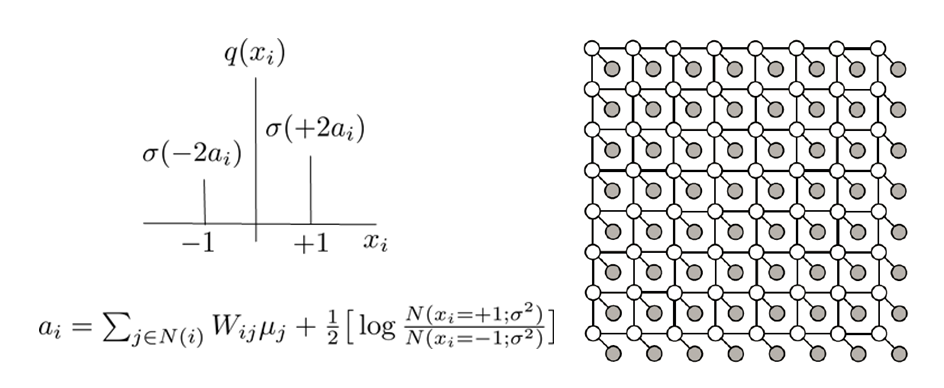
\includegraphics[width=0.8\textwidth, trim={10 10 10 10}]{figures/ising_vi1.png}
    \caption{Mean-field VI approximation (left) and Ising model (right).}
    \label{fig:ising_vi1}
\end{figure}

In order to compute this mean, we need to know the values of $q_j(x_j=+1)$ and $q_j(x_j=-1)$. Let $m_i = \sum_{j\in N(i)}w_{ij}\mu_j$ be the mean value of neighbors and let $L_{i}^{+} = N(x_i=+1,\sigma^2)$ and $L_{i}^{-} = N(x_i=-1, \sigma^2)$, then we can compute the mean as follows:
\begin{eqnarray}
    q_i(x_i=+1) &=& \frac{\exp \{m_i + L_{i}^{+}\}}{\exp \{m_i + L_{i}^{+}\} + \exp \{-m_i + L_{i}^{-}\}} \\
    &=& \frac{1}{1+\exp \{-2m_i + L_{i}^{-} - L_{i}^{+}\}} = \frac{1}{1+\exp \{-2a_i\}} = \sigma(2a_i)
\end{eqnarray}
where $a_i = m_i + 1/2(L_{i}^{+} - L_{i}^{-})$ and $\sigma(x)$ is a sigmoid function. Since $q_i(x_i=-1) = 1-q_i(x_i=+1)=1-\sigma(2a_i)=\sigma(-2a_i)$, we can write the mean of our variational approximation $q_i(x_i)$ as follows:
\begin{equation}
   \mu_i = E_{q_i}[x_i] = \sigma(2a_i) - \sigma(-2a_i) = \tanh(a_i)
\end{equation}
In other words, our mean-field updates of the variational parameters $\mu_i$ at iteration $k$ are computed as follows:
\begin{equation}
    \mu_{i}^{(k)} = \tanh \bigg(\sum_{j\in N(i)}w_{ij}\mu_{j}^{(k-1)} + \frac{1}{2}\bigg[\log \frac{N(x_i=+1,\sigma^2)}{N(x_i=-1,\sigma^2)} \bigg] \bigg)\times \lambda + (1-\lambda)\times \mu_{i}^{(k-1)}
\end{equation}
where we added a learning rate parameter $\lambda \in (0, 1]$. We further note that we can simplify the computation of ELBO term by term as follows:
\begin{eqnarray}
  && \sum_{(s,t)\in E} E_{q(x)}[x_s w_{st} x_t] = \frac{1}{2}\sum_{i=1}^{n}\sum_{j\in N(i)}\bigg(\sum_{x_i \in \{-1,+1\}} \sum_{x_j \in \{-1,+1\}}q_i(x_i)q_j(x_j)x_i J x_j \bigg) = \\
  && \frac{1}{2}\sum_{i=1}^{n}\sum_{j\in N(i)}\bigg(q_i(x_i=+1)JE[x_j] - q_i(x_i=-1)JE[x_j]\bigg) = \frac{1}{2}\sum_{i=1}^{n}\sum_{j \in N(i)} E[x_i] J E[x_j] 
\end{eqnarray}
Similarly,
\begin{eqnarray}
 && E_{q(x)}[\log N(x_i, \sigma^2)] = \sum_{i=1}^{n}\bigg[\sum_{x_i \in \{-1,+1\}}q_i(x_i)\log N(x_i,\sigma^2) \bigg] = \\
 && \sum_{i=1}^{n}\bigg[\sigma(2a_i)\log N(x_i=+1,\sigma^2)+\sigma(-2a_i)\log N(x_i=-1,\sigma^2) \bigg]
\end{eqnarray}

\begin{figure}[hptb]
    \centering
    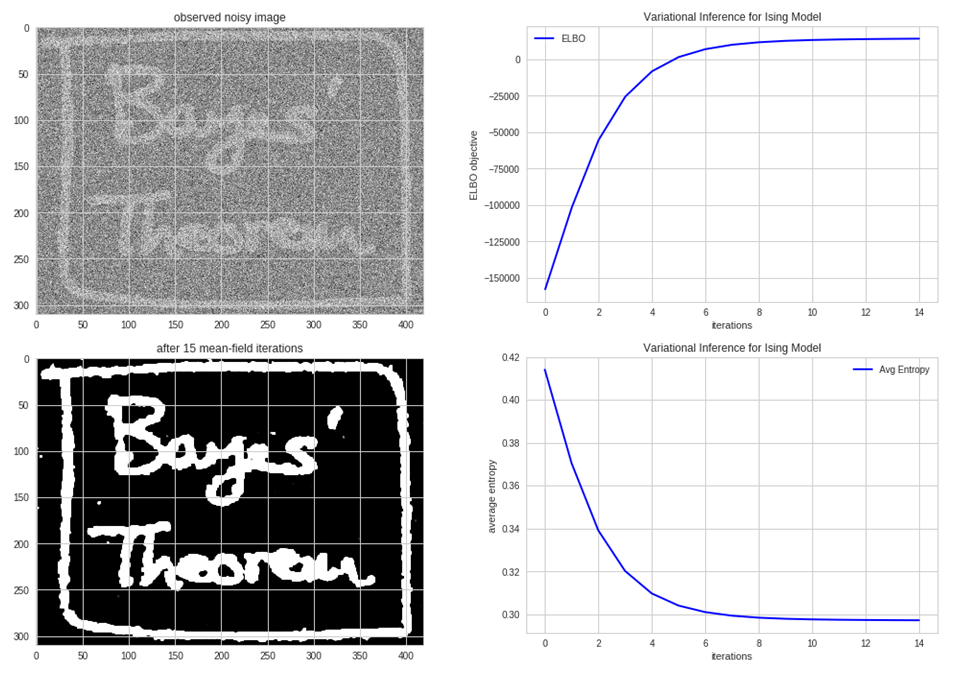
\includegraphics[width=0.8\textwidth, trim={10 10 10 10}]{figures/ising_vi2.png}
    \caption{Image Denoising for Ising model.}
    \label{fig:ising_vi2}
\end{figure}

Figure \ref{fig:ising_vi2} shows experimental results for binary image denoising via mean-field variational inference. The noisy observed image is shown in the top-left obtained by adding Gaussian noise to each pixel and binarizing the image based on mean threshold. We then set the variational inference parameters such as the coupling strength $J=1$, noise level $\sigma = 2$, smoothing rate $\lambda=0.5$ and max number of iterations to $15$. The resulting de-noised binary image is shown in the bottom-left corner of Figure \ref{fig:ising_vi2}. We can also see an increase in the ELBO objective (top-right) and a decrease in the average entropy of our binary random variables $q_i(x_i)$ representing the value of each pixel (bottom-right) as the number of mean-field iterations increases.\\

The 2-D Ising model can be extended in multiple ways, for example: 3-D grids and $K$-states per node (aka Potts model).\\

\subsection{Stochastic Variational Inference}

One limitation of LDA is that the number of topics is fixed ahead of time. A commonly used approach to finding the number of topics $K$ is cross-validation. However, for very large data-sets this approach may not be practical. We can address this issue with a Bayesian non-parametric topic model where the number of topics is learned from data: the Hierarchical Dirichlet Process (HDP) topic model.\\

\begin{figure}[tbhp]
    \centering
    \includegraphics[width=0.25\textwidth, trim={10 10 10 10}]{figures/local_global_gm.png}
    \caption{Graphical model with local and global latent variables.}
    \label{fig:svi_gm}
\end{figure}

While tranditional algorithms require repeatedly analyzing the whole data set before updating the variational parameters, we focus on analyzing randomly sampled subsets. First, we derive the Stochastic Variational Inference (SVI) algorithm for a class of graphical models with global and local laten variables as shown in Figure \ref{fig:svi_gm}. The join distribution factorizes into a product of a global term $\beta$ and local term $z_n$:
\begin{equation}
    p(x,z,\beta|\alpha) = p(\beta|\alpha)\prod_{n=1}^{N}p(x_n,z_n|\beta)
\end{equation}
Our goal is to approximate the posterior distribution of the hidden variables given the observations $p(\beta,z|x)$. We use a variational distribution to approximate the posterior as measured by KL divergence. Variational inference minimizes KL divergence or alternatively maximizes the evidence lower bound (ELBO):
\begin{eqnarray}
    \log p(x) &=& \log \int p(x,z,\beta) dz d\beta \\
              &=& \log \int p(x,z,\beta) \frac{q(z,\beta)}{q(z,\beta)} dz d\beta \\
              &=& \log \bigg(E_q \bigg[\frac{p(x,z,\beta)}{q(z,\beta)} \bigg] \bigg) \\
              &\geq& E_q[\log p(x,z,\beta)] - E_q[\log q(z,\beta)]\\
              &=& L(q)
\end{eqnarray}
The ELBO contains two terms: the first term is the expected log joint $E_q[\log p(x,z,\beta)]$ and the second term is the entropy of the variational distribution $- E_q[\log q(z,\beta)]$. We restrict $q(z,\beta)$ to be in a tractable family of distributions in order to efficiently compute the expectations in the ELBO. We then find the member of the family that maximizes the ELBO and use the optimized distribution as a proxy for the posterior. Solving this maximization problem is equivalent to finding the member of the family that is closest in KL divergence to the posterior:
\begin{eqnarray}
    \min KL(q(z,\beta)||p(z,\beta|x)) &=& E_q[\log q(z,\beta)] - E_q[\log p(z,\beta|x)] \\
    &=& E_q[\log q(z,\beta)] - E_q[\log p(x,z,\beta)] + \log p(x) \\
    &=& -L(q) + \mathrm{const}
\end{eqnarray}
where $\log p(x)$ is replaces by a constant because it does not depend on $q$. The simplest variational family of distributions is the fully factored mean-field family. In this family, each hidden variable is independent and governed by its own parameter:
\begin{equation}
    q(z,\beta) = q(\beta|\lambda)\prod_{n=1}^{N}\prod_{j=1}^{J}q(z_{nj}|\phi_{nj})
\end{equation}
To specify the form of the distribution, we choose $q(\beta|\lambda)$ and $q(z_{nj}|\phi_{nj})$ to be in the exponential distribution with the natural parameters $\lambda$ and $\phi_{nj}$:
\begin{eqnarray}
   q(\beta|\lambda) &=& h(\beta)\exp\{\lambda^{T}t(\beta) - a_{g}(\lambda)\}\\
   q(z_{nj}|\phi_{nj}) &=& h(z_{nj})\exp\{\phi_{nj}^{T}t(z_{nj} - a_{l}(\phi_{nj}))\}
\end{eqnarray}
The mean-field family has several computational advantages. For example the entropy term in the ELBO objective function decomposes:
\begin{equation}
   -E_q[\log q(z,\beta)] = -E_{\lambda}[\log q(\beta)] - \sum_{n=1}^{N}\sum_{j=1}^{J}E_{\phi_{nj}}[\log q(z_{nj})]
\end{equation}
In traditional mean-field variational inference, we maximize $L(q)$ with coordinate ascent: we iteratively optimize each variational parameter while holding the other parameters fixed. Given our assumptions that each conditional is an exponential family, we can optimize each coordinate in closed form. We first derive the coordinate update for the global parameter $\lambda$. Keeping only the terms of $L(q)$ that depend on $\lambda$, we get:
\begin{eqnarray}
    L(\lambda) &=& E_q[\log p(x,z,\beta)] - E_q[\log q(\beta)] + \mathrm{const} \\
    &=& E_q[\log p(\beta|x,z)] - E_q[\log q(\beta)] + \mathrm{const}
\end{eqnarray}
where we used the factorization $p(x,z,\beta) = p(\beta|x,z)p(x,z)$ and absorbed $E_q[p(x,z)]$ into the constant that does not depend on $\lambda$. To derive the coordinate ascent update, we take the gradient \cite{SVI2013}:
\begin{equation}
   \nabla_{\lambda}L = \nabla_{\lambda}^{2}a_g(\lambda)(E_q[\eta_g(x,z,\alpha)] - \lambda) 
\end{equation}
We can set the gradient to zero by setting $\lambda = E_q[\eta_g(x,z,\alpha)]$. This sets the global variational parameter equal to the expected natural parameter of its complete conditional distribution. We now turn to the local parameters $\phi_{nj}$. The gradient is similar to the global case:
\begin{equation}
   \nabla_{\phi_{nj}}L = \nabla_{\phi_{nj}}^{2}a_{l}(\phi_{nj})(E_q[\eta_l(x_n,z_{n,-j},\beta)] - \phi_{nj})
\end{equation}
We can set the gradient to zero by choosing $\phi_{nj} = E_q[\eta_l(x_n,z_{n,-j},\beta)]$. The variational updates form the algorithm for coordinate ascent variational inference, iterating between updates of each local parameter and the global parameter. The full algorithm is described in Algorithm \ref{alg:svi_1} which is guaranteed to find a local optimum of the ELBO.\\

\begin{algorithm}
\caption{Coordinate Ascent SVI \cite{SVI2013}}
\label{alg:svi_1}
\begin{algorithmic}[1]
\STATE Initialize $\lambda^{(0)}$ randomly
\STATE \textbf{repeat}
\STATE ~~~ \textbf{for} each local variational parameter $\phi_{nj}$ \textbf{do}
\STATE ~~~ ~~~ Update $\phi_{nj}^{(t)} = E_{q^{(t-1)}}[\eta_{l,j}(x_n,z_{n,-j},\beta)]$
\STATE ~~~ \textbf{end for}
\STATE ~~~ Update the global variational parameters: $\lambda^{(t)} = E_{q^{(t)}}[\eta_g(z,x)]$
\STATE \textbf{until} the ELBO converges
\end{algorithmic}
\end{algorithm}

We now turn the Hierarchical Dirichlet Process (HDP) topic model. The HDP topic model couples a set of document-level DPs via a single top-level DP \cite{teh2005jasa}. The base distribution $H$ of the top-level DP is a symmetric Dirichlet over the vocabulary simplex. We draw once from this DP: $G_0 \sim DP(\omega, H)$. In the second level, we use $G_0$ as a base measure for a document level DP: $G_d \sim DP(\alpha, G_0)$. As a result, the global topics are shared between documents with different mixing proportions.

\begin{figure}[tbhp]
    \centering
    \includegraphics[width=0.5\textwidth, trim={10 10 10 10}]{figures/hdp_svi_gm.png}
    \caption{HDP graphical model for SVI inference.}
    \label{fig:svi_gm2}
\end{figure}

Figure \ref{fig:svi_gm2} shows a graphical model for the HDP topic model. The generative process of the HDP topic model can be described as follows.
\begin{enumerate}
    \item Draw global topics, $\beta_k \sim \mathrm{Dir}(\eta)$
    \item Draw mixing proportions, $\nu_k \sim \mathrm{Beta}(1,\omega)$
    \item For each document $d$:
    \begin{enumerate}
        \item Draw document-level topic indices, $c_{di} \sim \mathrm{Mult}(\nu)$
        \item Draw document-level mixing proportions, $\pi_{di} \sim \mathrm{Beta}(1,\alpha)$
        \item For each word $n$:
        \begin{enumerate}
            \item Draw topic assignment $z_{dn} \sim \mathrm{Mult}(\pi_d)$
            \item Draw word $w_n \sim \mathrm{Mult}(\beta_{c_{d,z_{dn}}})$
        \end{enumerate}
    \end{enumerate}
\end{enumerate}

In order to implement an infinite number of topics at corpus and document levels we need to truncate our representation to $K$ topics at the corpus level and $T$ topics at the document level. This ways we are optimizing a finite number of variational parameters. We can write down the joint variational family distribution as:
\begin{equation}
    q(\beta,\nu,z,\pi) = \bigg(\prod_{k=1}^{K}q(\beta_k|\lambda_k)q(\nu_k|a_k)\bigg)\bigg(\prod_{d=1}^{D}\prod_{i=1}^{T}q(c_{di}|\zeta_{di})q(\pi_{di}|\gamma_{di})\prod_{n=1}^{N}q(z_{dn}|\phi_{dn}) \bigg)
\end{equation}
The Stochastic Variational Inference (SVI) algorithm is summarized in Algorithm \ref{alg:svi_2}.

\begin{algorithm}
\caption{Stochastic Variational Inference for HDP \cite{SVI2013}}
\label{alg:svi_2}
\begin{algorithmic}[1]
\STATE Initialize $\lambda^{(0)}$ randomly. Set $a^{(0)}=1$ and $b^{(0)}=\omega$
\STATE Set the step-size schedule $\rho_t$
\STATE \textbf{repeat}
\STATE ~~~ Sample a document $w_d$ uniformly from the dataset
\STATE ~~~ For $i \in \{1,...,T\}$, $k \in \{1,...,K\}$: $\zeta_{di}^{k} \propto \exp \{\sum_{n=1}^{N}E[\log \beta_{k,w_{dn}}]\}$
\STATE ~~~ For $n \in \{1,...,N\}$, $i \in \{1,...,T \}$: $\phi_{dn}^{i} \propto \exp\{\sum_{k=1}^{K}\zeta_{di}^{k}E[\log\beta_{k,w_{dn}}]\}$
\STATE ~~~ \textbf{repeat}
\STATE ~~~ ~~~ For $i \in \{1,...,T\}$ set \\
~~~ ~~~ ~~~ ~~~ $\gamma_{di}^{(1)} = 1 + \sum_{n=1}^{N}\phi_{dn}^{i}$\\
~~~ ~~~ ~~~ ~~~ $\gamma_{di}^{(2)} = \alpha + \sum_{n=1}^{N}\sum_{j=i+1}^{T}\phi_{dn}^{j}$\\
~~~ ~~~ ~~~ ~~~ $\zeta_{di}^{k} \propto \exp \{E[\log \sigma_k(V)]+\sum_{n=1}^{N}\phi_{dn}^{i}E[\log \beta_{k,w_{dn}}] \}$, $k \in \{1,...,K\}$
\STATE ~~ ~~~ For $n \in \{1,...,N\}$ set \\
~~~ ~~~ ~~~ ~~~ $\phi_{dn}^{i} \propto \exp \{E[\log \sigma_i(\pi_d)]+\sum_{k=1}^{K}\zeta_{di}^{k}E[\log \beta_{k,w_{dn}}] \}$, $i \in \{1,...,T\}$
\STATE ~~~ \textbf{until} local parameters converge
\STATE ~~~ For $k \in \{1,...,K\}$ set intermediate topics:\\
~~~ ~~~ ~~~ ~~~ $\hat{\lambda}_{kv} = \eta + D\sum_{i=1}^{T}\zeta_{di}^{k}\sum_{n=1}^{N}\phi_{dn}^{i}w_{dn}$\\
~~~ ~~~ ~~~ ~~~ $\hat{a}_k = 1 + D\sum_{i=1}^{T} \zeta_{di}^{k}$\\
~~~ ~~~ ~~~ ~~~ $\hat{b}_k = \omega + D\sum_{i=1}^{T}\sum_{l=k+1}^{K}\zeta_{di}^{l}$
\STATE ~~~ Set \\
~~~ ~~~ ~~~ ~~~ $\lambda^{(t)} = (1-\rho_t)\lambda^{(t-1)} + \rho_t\hat{\lambda}$\\
~~~ ~~~ ~~~ ~~~ $a^{(t)} = (1-\rho_t)a^{(t-1)} + \rho_t\hat{a}$\\
~~~ ~~~ ~~~ ~~~ $b^{(t)} = (1-\rho_t)b^{(t-1)} + \rho_t\hat{b}$
\STATE \textbf{until} end of documents
\end{algorithmic}
\end{algorithm}
where the expectations used in Algorithm \ref{alg:svi_2} are computed as follows:
\begin{eqnarray}
    E[\log \beta_{kv}] &=& \Psi(\lambda_{kv}) - \Psi(\sum_{v^{\prime}}\lambda_{kv^{\prime}})\\
    E[\log \sigma_k(V)] &=& \Psi(a_k) - \Psi(a_k+b_k) + \sum_{l=1}^{k-1}[\Psi(b_l)-\Psi(a_l+b_l)]
\end{eqnarray}

The on-line variational inference algorithm for Hierarchical Dirichlet Process was used to fit a topic model on the 20newsgroups dataset. The dataset consists of $11,314$ documents and over $100K$ unique tokens. Standard text pre-processing was used including tokenization, stop-word removal and stemming. A compressed dictionary of $4K$ words was constructed by filtering out tokens that appear in less than $5$ documents and more than $50\%$ of the corpus. The top-level truncation was set to $T=20$ topics and the second level truncation was set to $K=8$ topics. The concentration parameters were chosen as $\gamma = 1.0$ at the top-level and $\alpha=0.1$ at the group level to yield a broad range of shared topics that are concentrated at the group level. Figure \ref{fig:hdp_topics_vb} shows a sample of the global level topics inferred by online variational HDP algorithm. We can find topics about autos, politics and for sale items that correspond to the target labels of the 20newsgroups dataset.

\begin{figure}[thpb]
    \centering
    \includegraphics[width=0.8\textwidth, trim={10 10 10 10}]{figures/hdp_topics.png}
    \caption{Sample of HDP topics inferred using online variational bayes algorithm on 20newsgroups dataset.}
    \label{fig:hdp_topics_vb}
\end{figure}

\subsection{Normalizing Flows}

A normalizing flow describes the transformation of a probability density through a sequence of invertible mappings \cite{Rezende2015}. The target density is approximated through a flow of the prior distribution through a sequence of invertible (one-to-one) transformations resulting in the target posterior density.\\

The basic rule for transformation of densities considers an invertible, smooth mapping $f: \mathbb{R}^{d}\rightarrow \mathbb{R}^{d}$. Recall, that in the case of discrete random variables, for a one-to-one $y=f(x)$ where $X \sim p(x)$, the transformed density is $p_y(y) = \sum_{\{x : y = f(x)\}} p_x(x)$. If $X$ is a continuous random variable, we can differentiate the CDF to obtain an expression for the transformed density:
\begin{eqnarray}
   F_{y}(y) &=& P(Y \leq y) = P(f(X) \leq y) = P(X \leq f^{-1}(y)) \\
   p_{y}(y) &=& \frac{d}{dy}F_{y}(y) = \frac{d}{dy}P(X \leq f^{-1}(y)) = \frac{dx}{dy}\frac{d}{dx}P(X \leq f^{-1}(y)) = p_x(x)|\frac{dx}{dy}|
\end{eqnarray}
The above expression generalizes for high dimensional transformations using a Jacobian:
\begin{equation}
    p_y(y) = p_x(x)|\mathrm{det}\bigg(\frac{\partial x}{\partial y}\bigg)|
\end{equation}
Let's examine a $k$ step transformation:
\begin{equation}
    z_k = f_k \circ f_{k-1} \circ \cdots \circ f_{2} \circ f_{1} (z_0) = f_k(f_{k-1}(\cdots f_{2}(f_{1}(z_0))))
\end{equation}
For $k=1$, we have $z_1 = f_{1}(z_0)$, where $z_0 \sim q_{0}(z_0)$ and
\begin{equation}
   q_{1}(z_1) = q_{0}(z_0)|\mathrm{det}\bigg(\frac{\partial z_0}{\partial z_1}\bigg)|  = q_{0}(z_0)|\mathrm{det}\bigg(\frac{\partial f_{1}^{-1}}{\partial z_1}\bigg)| = q_{0}(z_0)|\mathrm{det}\bigg(\frac{\partial f_{1}}{\partial z_0}\bigg)|^{-1}  
\end{equation}
For $k=2$, we have $z_2 = f_2 \circ f_1 (z_0) = f_2(f_1(z_0)) = f_2(z_1)$ that we can re-write as:
\begin{equation}
    q_{2}(z_2) = q_1(z_1)|\mathrm{det}\bigg(\frac{\partial f_2}{\partial z_1} \bigg)|^{-1} =  q_{0}(z_0)|\mathrm{det}\bigg(\frac{\partial f_{1}}{\partial z_0}\bigg)|^{-1} \times |\mathrm{det}\bigg(\frac{\partial f_2}{\partial z_1} \bigg)|^{-1} 
\end{equation}
Generalizing for $k$ steps, we have:
\begin{equation}
    q_{k}(z_k) = q_{0}(z_0)|\mathrm{det}\bigg(\frac{\partial f_{1}}{\partial z_0}\bigg)|^{-1} \times |\mathrm{det}\bigg(\frac{\partial f_2}{\partial z_1} \bigg)|^{-1} \times \cdots \times |\mathrm{det}\bigg(\frac{\partial f_k}{\partial z_{k-1}}\bigg)|^{-1} 
\end{equation}
Taking the log, we can represent this compactly as:
\begin{equation}
    \log q(z_k) = \log q(z_0) - \sum_{i=1}^{K}\log|\mathrm{det}\bigg(\frac{\partial f_i}{\partial z_{i-1}}\bigg)|
\end{equation}
Note the above density is parametrized by one-to-one, invertible transformations $f_k(\cdot)$. In order to learn the flow parameters, we consider the following variational inference objective.
\begin{equation}
    \log p(x) \geq E_q\big[\log \frac{p(x,z)}{q(z|x)} \big] = \mathrm{ELBO} = -F(x)
\end{equation}
Thus, we are interested in maximizing the ELBO or equivalently minimizing the free energy $F(x)$. Treating $F(x)$ as a loss function, we can expand it as follows:
\begin{eqnarray}
    &&\min F(x) = E_{q(z|x)}\bigg[\log \frac{q(z|x)}{p(x,z)} \bigg] = E_{q_0(z_0)}\bigg[\log q_k(z_k) - \log p(x, z_k)\bigg] \nonumber \\
 &=& E_{q_0(z_0)}\bigg[\log q_0(z_0)\bigg] - E_{q_0(z_0)}\bigg[\sum_{k=1}^{K}\log|\det\bigg(\frac{\partial f_i}{\partial z_{i-1}} \bigg)|\bigg] - E_{q_0(z_0)}\bigg[\log p(x, z_k)\bigg]
\end{eqnarray}
where $E_{q_0(z_0)}$ is Monte Carlo expectation with respect to the prior distribution $q_0(z)$. Note that we can ignore the first term in the objective function because it doesn't depend on the flow paramters. Also, we swapped the expectation wrt to $q(z)$ to an expectation with respect to the prior $q_0(z)$, this is true in general for normalizing flows since we can fix the flow parameters and can compute expectations with respect to any of the intermediate distributions by drawing samples from the prior:
\begin{eqnarray}
    E_{q_k}[h(z)] &=& \int q_k(z)h(z) dz = \frac{1}{n}\sum_{i=1}^{n} h(z_{i}^{k}),~~~\mathrm{where}~~~z_{i}^{k} \sim q_k(z) \\
    &=& \frac{1}{n}\sum_{i=1}^{n}h(f_k \circ f_{k-1} \circ \cdots \circ f_1(z_{i}^{0})), ~~~\mathrm{where}~~~z_{i}^{0} \sim q_0(z) \\
    &=& E_{q_0}[h(f_k \circ f_{k-1} \circ \cdots \circ f_1(z_{i}^{0}))]
\end{eqnarray}

For NF inference, we need to identify a class of invertible transformations and efficient algorithms for computing determinant of the Jacobian. \textit{Planar} and \textit{radial} flows were designed in a way that makes their determinant of Jacobian easy to compute. Other extensions include auto-regressive flows. A planar transform can be defined as follows:
\begin{equation}
    f(z) = z + uh(w^{t}z + b)
\end{equation}
parameterized by $\lambda = \{w \in \mathbb{R}^{d}, u \in \mathbb{R}^{d}, b \in \mathbb{R}\}$, where $h$ is a smooth, point-wise non-linearity (such as $\tanh$) with derivative $h^{\prime}$. For a planar flow of this form, we can compute the logdet Jacobian term in $O(D)$ time:
\begin{equation}
    |\det \frac{\partial f}{\partial z}| = |\det (I + uh^{\prime}(w^{t}z + b)w^{t})| = |1 + u^{t}h^{\prime}(w^{t}z + b)w|
\end{equation}
As a result, we are interested in optimizing the non-convex objective:
\begin{equation}
    \min_{\{w_k,u_k,b_k\}} - E_{q_0}\bigg[\sum_{k=1}^{K} \log |1 + u_{k}^{t}h^{\prime}(w_{k}^{t}z_{k-1} + b_k)w_k|\bigg] - E_{q_0}\bigg[\log p(x, z_k)\bigg]
\end{equation}

Alternatively, we can consider a family of transformations that modify an initial density $q_0$ around a reference point $z_0$, known as a radial flow:
\begin{equation}
    f(z) = z + \beta h(\alpha, r)(z-z_0)
\end{equation}
where $r = |z-z_0|$ and $h(\alpha, r) = 1/(\alpha + r)$ and the parameters of the map are $\lambda = \{z_0 \in \mathbb{R}^{d}, \alpha \in \mathbb{R}^{+}, \beta \in \mathbb{R}\}$. This family also allows for linear computation of the determinant:
\begin{equation}
    |\det \frac{\partial f}{\partial z}| = [1+\beta h(\alpha,r)]^{d-1}[1 + \beta h(\alpha,r) + \beta h^{\prime}(\alpha, r)r]
\end{equation}

The effect of invertible flows can be understood as a sequence of expansions or contractions on the initial density. The resuling distribution is transformed by increasing density outside its original region (expansion) or concentrating in its original region (contraction). With an appropriate choice of transformation $f_k$ we can use a simple prior distribution such as factorized Gaussian and by applying normalizing flows of different lengths, we obtain increasingly complex and multi-modal distributions. One question one may ask is how to choose $K$ the length of the flow that invites a non-parametric way of looking at normalizing flows.\\

\subsubsection{Annealed NF}

Annealed Normalizing Flows explores the hypothesis that if we don't take the steepest descent path but take one guided by AIS, we can arrive at a better solution (non-greedy). The annealed NF algorithm is summarized in Algorithm \ref{alg:annealed_nf}\\

\begin{algorithm}
\caption{Annealed Normalizing Flows}
\label{alg:annealed_nf}
\begin{algorithmic}[1]
\STATE Initialize $\phi$ randomly
\STATE \textbf{for} $t = 1$ to $T$ \textbf{do} 
\STATE ~~~ $x_0 \sim N(0, I)$ //sample a mini-batch of data of size m
\STATE ~~~ $x_k = f_k \circ f_{k-1} \circ \cdots \circ f_1(x_0)$ //NF forward pass
\STATE ~~~ $\beta_t = \beta(t, a) = 1-\exp \big(-at\big)$ //update beta
\STATE ~~~ $\log p_t(x_k) = (1-\beta_t)\log N(0, I) + \beta_t \log p(x_k)$ //compute annealed target distribution
\STATE ~~~ $\log q(x_k; \phi) = \log q(z_0) - \sum_{i=1}^{K}\log | \det \bigg(\frac{\partial f_i}{\partial x_{i-1}} \bigg)|$ //compute variational approximation
\STATE ~~~ $\mathrm{Loss}(x_k) = E_{q0}\bigg[\log q(x_k; \phi) - \log p_t(x_k)\bigg]$ // compute variational loss (negative ELBO)
\STATE ~~~ $\phi = \phi - \epsilon_t \times g$, where $g = \frac{1}{m}\sum_{i=1}^{m}\nabla_{\phi}\mathrm{Loss}(x_{k}^{(i)}; \phi)$ //update NF parameters (backward pass)
\STATE \textbf{end for}
\end{algorithmic}
\end{algorithm}

Geometric average of the prior and target distributions used to create an intermediate $p_t(x_k)$ minimizes a weighted sum of the KL divergences to the prior $p_a$ and target $p_b$:
\begin{eqnarray}
    p_t(x_k) &=& \arg \min_q (1-\beta)D_{KL}(q||p_a) + \beta D_{KL}(q||p_b) \\
    && \mathrm{s.t.}~\sum_x q(x) = 1
\end{eqnarray}
The objective function above is minimized by $p_t(x_k)$ that allocates mass in the intersection of $p_a$ and $p_b$ (due to reverse KL), i.e. $p_t(x_k)$ is high in regions that are likely under both the prior and the target distributions as shown in Figure \ref{fig:ga_ma_path}. To see why the expression above is true we can include the constraints as part of the objective and optimize the Lagrangian:
\begin{eqnarray}
    L(q) &=& \lambda(1-\sum_x q(x)) + (1-\beta)\sum_x q(x)\big[\log q(x) - \log p_a(x)\big] \nonumber \\
         &+& \beta\sum_x q(x) \big[\log q(x) - \log p_b(x)\big] \\
         &=& \lambda(1-\sum_x q(x)) + \sum_x q(x) \log q(x) \nonumber \\
         &-& \sum_x q(x)\big[(1-\beta)\log p_a(x) + \beta \log p_b(x)\big]
\end{eqnarray}
By taking the derivative of $L(q)$ and setting it to zero, we get:
\begin{eqnarray}
    \frac{d L(q)}{d q(x)} &=& -\lambda + \log q(x) + 1 - \big[(1-\beta)\log p_a(x) + \beta \log p_b(x)\big] = 0 \\
    \log q(x) &=& \lambda - 1 + \log p_{a}^{1-\beta}(x) + \log p_{b}^{\beta}(x) \\
    q(x) &\propto& p_{a}^{1-\beta}(x)p_{b}^{\beta}(x)
\end{eqnarray}
for some constant $\lambda$, s.t. $\sum_x q(x) = 1$. If $p_a$ and $p_b$ belong to an exponential family $P$ with natural parameters $\theta_{p_a}$ and $\theta_{p_b}$, the optimum distribution is also in exponential family with natural parameters $\theta_{\beta} = (1-\beta)\theta_{p_a} + \beta\theta_{p_b}$.\\

\begin{figure}[thpb]
    \centering
    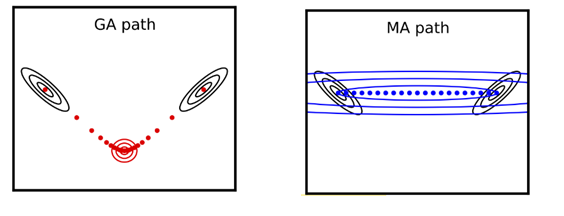
\includegraphics[width=0.4\textwidth, trim={10 10 10 10}]{figures/ga_ma_path.png}
    \caption{Geometric Average (GA) path (left) and Moment Average (MA) path (right). Figure source: \cite{Grosse2013}.}
    \label{fig:ga_ma_path}
\end{figure}

If instead we minimize the forward KL objective with respect to natural parameters $\theta$ of the approximating distribution, we obtain the Moment Average (MA) path \cite{Grosse2013}. 
\begin{equation}
    \arg \min_\theta (1-\beta)D_{KL}(p_a||q(x;\theta)) + \beta D_{KL}(p_b||q(x;\theta))
\end{equation}
We can re-write the objective as follows:
\begin{eqnarray}
    J(\theta) &=& (1-\beta)\sum_x p_a(x)\big[\log p_a(x) - \log q(x;\theta) \big] \nonumber \\
    &+& \beta \sum_x p_b(x)\big[\log p_b(x) - \log q(x;\theta)\big] \\
    &=& \mathrm{const} - \sum_{x}\big[(1-\beta)p_a(x) + \beta p_b(x)]\log q(x) \\
    &=& \mathrm{const}^{\prime} + \log Z(\theta) - \sum_x\big[(1-\beta)p_a(x)+\beta p_b(x)\big]\theta^{T}\phi(x)
\end{eqnarray}
By setting the derivative to zero, we get:
\begin{eqnarray}
    \frac{\partial J(\theta)}{\partial \theta_i} &=& E_q[\phi_i(x)] - \sum_x\big[(1-\beta)p_a(x)+\beta p_b(x)\big]\phi_i(x) = 0 \\
    E_q[\phi_i(x)] &=& (1-\beta)E_{p_a}[\phi_i(x)] + \beta E_{p_b}[\phi_i(x)]
\end{eqnarray}
The above expression can be interpreted as drawing $(1-\beta)$ fraction of points from $p_a$ and $\beta$ fraction of points from $p_b$. Notice that because we are optimizing the forward KL, the approximating distribution includes the support of both $p_a$ and $p_b$ as shown in Figure \ref{fig:ga_ma_path}. 

\subsubsection{NF experiments}

To evaluate how well NF can approximate posterior densities, we designed the following experiment. Let $p(x) \propto \exp\{-E(x)\}$ be our target distribution with energy $E(x)$ defined as follows:
\begin{equation}
    E(x) = \frac{1}{2}\bigg(\frac{||z||-2}{0.4}\bigg)^{2} - \log \bigg(e^{-\frac{1}{2}\big[\frac{z_1-2}{0.6}\big]^{2}} + e^{-\frac{1}{2}\big[\frac{z_1+2}{0.6}\big]^{2}} \bigg)
\end{equation}
We restrict ourselves to $K$ planar flows and define the training epoch to be $512$ iterations with a mini-batch size of $512$ samples drawn from standard normal prior. The NF algorithm is implemented in PyTorch using CUDA GPU. 

\begin{figure}[thpb]
    \centering
    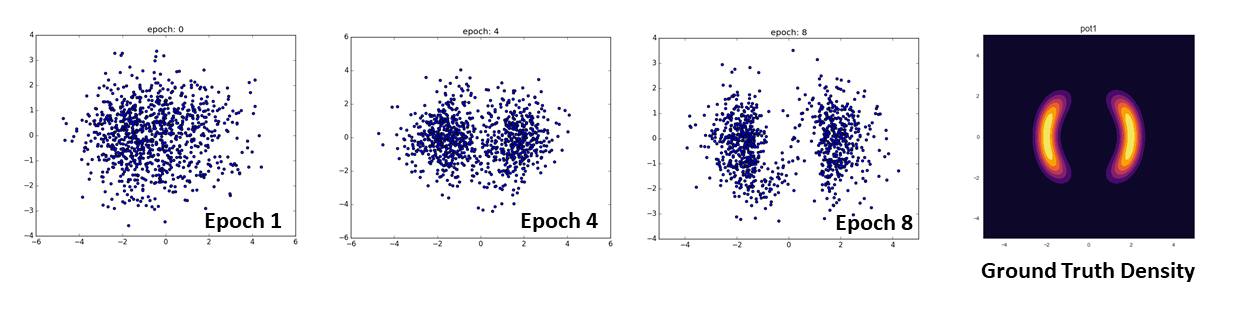
\includegraphics[width=\textwidth, trim={10 10 10 10}]{figures/nf_exp1.png}
    \caption{Samples from NF approximation to ground truth density.}
    \label{fig:nf_exp1}
\end{figure}

Figure \ref{fig:nf_exp1} shows samples drawn from NF model trained to minimize the free energy loss $F(x)$:
\begin{equation}
    \log p(x) \geq E_q\bigg[\log \frac{p(x,z)}{q(z|x)}\bigg] = \mathrm{ELBO} = -F(x)
\end{equation}
We can see that as the number of iterations progresses the NF approximations starts to resemble the ground truth density.\\

Since the ground truth density is $2$ dimensional, we can compute the ground truth value of $\log p(x)$ using numerical integration as well as Annealed Importance Sampling (AIS).

\begin{figure}[thpb]
    \centering
    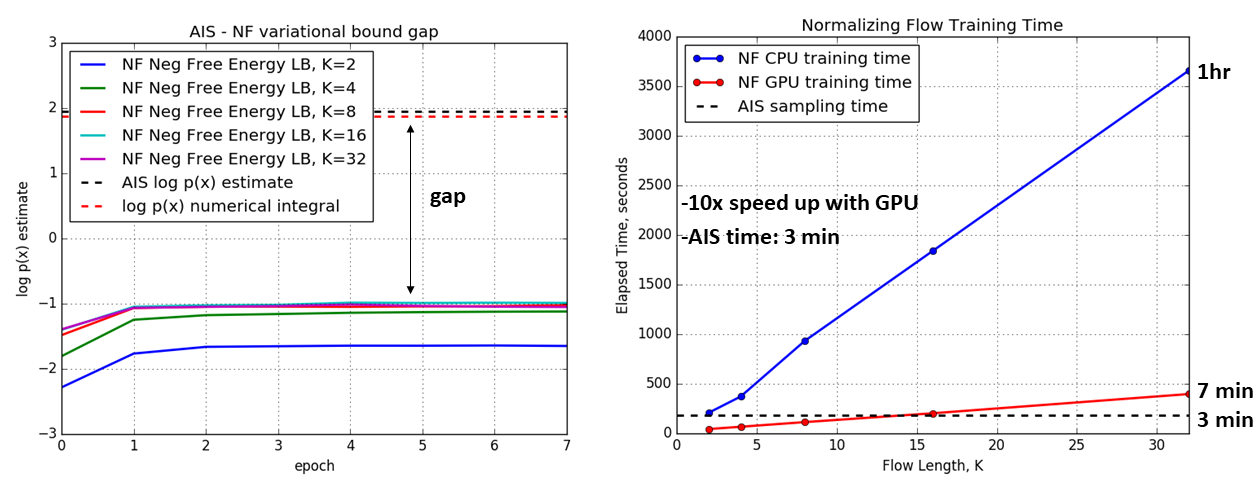
\includegraphics[width=0.9\textwidth, trim={10 10 10 10}]{figures/nf_exp2.png}
    \caption{NF variational objective gap (left). NF timing experiments (right).}
    \label{fig:nf_exp2}
\end{figure}

Figure \ref{fig:nf_exp2} (left) shows the variational objective gap between the negative free energy and the ground truth value estimated by numerical integration:
\begin{equation}
    \log p(x) = \mathrm{ELBO} + D_{KL}(q(z)||p(z|x))
\end{equation}
We can see that as we increase the number of planar flows $K$, we get a more accurate representation of the posterior. Timing experiments in Figure \ref{fig:nf_exp2} (right) show that GPU provides about $10x$ speed up in comparison with CPU and linear increase with the number of flows $K$. 






